\begin{frame}[c]{Apresentação}
    \begin{itemize}
        \item Professor Rodrigo de Farias Gomes
        \item Telefone (somente mensagens): (92) 9 9405-1724
        \item E-mail: shpnft@gmail.com
    \end{itemize}
\end{frame}

\begin{frame}{Ementa de Geometria Analítica}
    \begin{itemize}
        \item Vetores no plano e no espaço
        \item Operações com vetores: adição, multiplicação por escalar e produto interno
        \item Produto interno, produto vetorial e produto misto
        \item Equação vetorial de uma reta
        \item Equação do plano
        \item Distância entre ponto e plano, entre reta e plano e entre planos 
        \item Interpretação geométrica de sistemas de equações lineares com duas incógnitas
        \item Sistemas equações lineares e seu significado geométrico
        \item Equações reduzidas da elipse, hipérbole e parábola
        \item Quádricas 
    \end{itemize}
\end{frame}

\begin{frame}{Avaliação}
    \begin{itemize}
        \item A avaliação será na forma de 3 notas: \(N_1\), \(N_2\) e \(N_3\)
        \item A média dos exercícios escolares (\(MEE\)) será dada por
            \[
                MEE=\frac{N_1+N_2+N_3}{4}
            \]
        \item Se \(MEE \geq 8,0\), então a média final (\(MF\)) será igual à \(MEE\)
        \item Se \(MEE < 8,0\), então
            \[
                MF=\frac{2\times MEE+PF}{3}
            \]
            onde PF é a nota da \textbf{prova final}
        \item Se \(MF \geq 5,0\) e a frequência em sala for maior que 75\%, o aluno está aprovado
    \end{itemize}
\end{frame}

\begin{frame}{Livro Texto}
   \begin{center}
       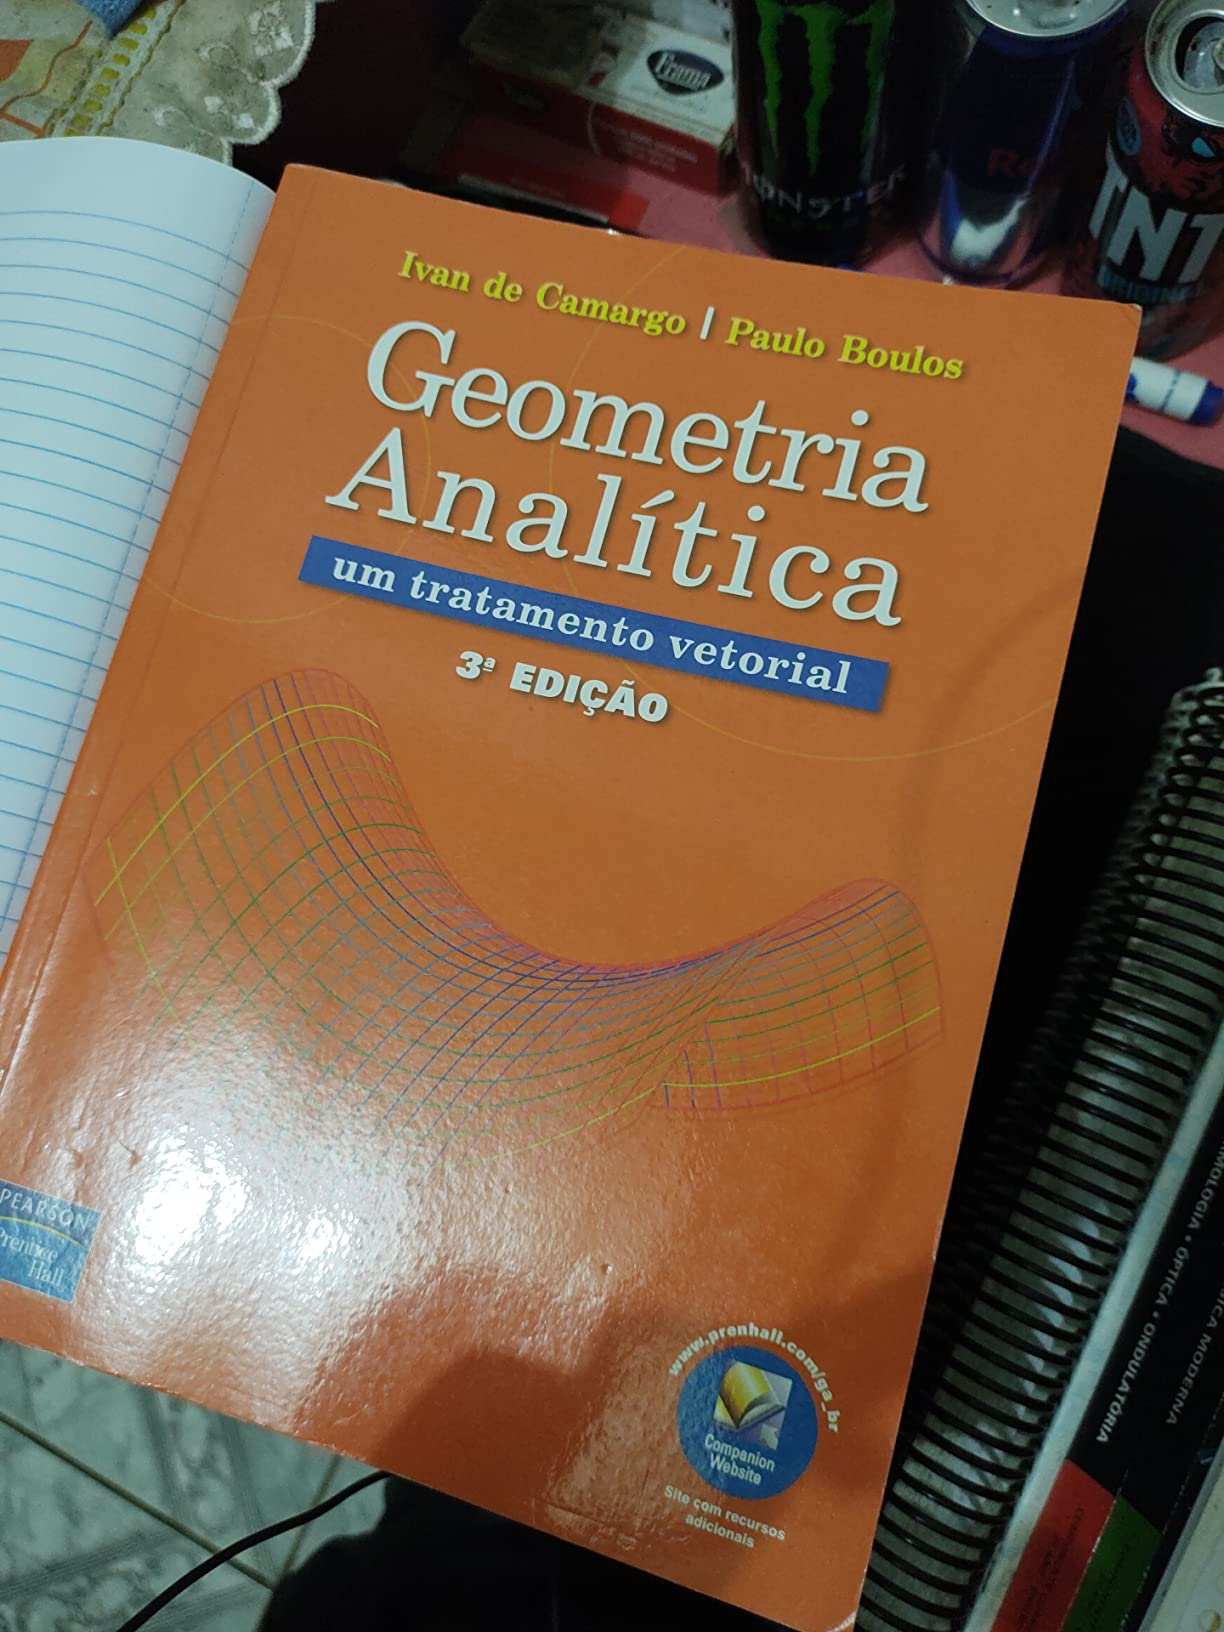
\includegraphics[height=0.8\textheight]{images/livro-texto}
   \end{center} 
\end{frame}

\begin{frame}{Geometria plana}
    \begin{itemize}
        \item Ponto
        \item Reta        
            \begin{itemize}
                \item Segmento de reta
            \end{itemize}
        \item Plano
        \item Polígonos 
            \begin{itemize}
                \item Triângulos
                \item Quadriláteros (quadrado, paralelogramo, losango)
                \item Pentágonos, hexágonos etc 
                \item<2> Perímetro e área
            \end{itemize}
        \item Círculo
            \begin{itemize}
                \item Circunferência
                \item Cordas
                \item Arcos
                \item<2> Raio, diâmetro, comprimento e área
            \end{itemize}
    \end{itemize}
\end{frame}

\begin{frame}{Nomenclatura e notação}
    \begin{itemize}[<+->]
        \item Dois pontos distintos \(A\) e \(B\) do espaço determinam uma reta \(r\) 
        \item O segmento de reta entre \(A\) e \(B\) é a parte da reta compreendida entre esses dois pontos
        \item O \textbf{segmento orientado} com origem \(A\) e extremidade \(B\) será indicado por \((A,B)\)
        \item Vamos considerar os pontos como segmentos orientados sem ''tamanho'' (nulos)
        \item Ou seja, o ponto \(A\) pode ser identificado como o segmento orientado \((A,A)\)
        \item O segmento orientado \((A,B)\) é \textbf{equipolente} ao segmento orientado \((A',B')\) se:
            \begin{itemize}[<.->]
                \item forem ambos nulos ou
                \item tiverem a mesma direção, mesmo comprimento e mesmo sentido
            \end{itemize}
        \item Indica-se a equipolência entre \((A,B)\) e \((A',B')\) por 
            \[
                (A,B) \sim (A',B')
            \]
    \end{itemize}
\end{frame}

\begin{frame}{Vetores}
    \begin{itemize}
        \item<+-> O \textbf{vetor} determinado por um segmento orientado \((A,B)\) é o conjunto de todos os segmentos orientados 
            do espaço que são \textbf{equipolentes} ao segmento orientado \((A,B)\)
        \item<.-> O vetor determinado por \((A,B)\) pode ser indicado por \(\vec{AB}\) ou por uma letra minúscula quando não se
            quer destacar um representante (por exemplo, \(\vec{a}\))
        \item<+-> Note que \((A,B)\) não é a mesma coisa de \(\vec{AB}\): um vetor pode ser representado por uma infinidade 
            de segmentos orientados distintos
        \item<.-> Se \((A,B) \sim (A',B')\), então \(\vec{AB} = \vec{A'B'}\) mesmo que \((A,B) \neq (A',B')\)
        \item<+-> \textbf{Vetor nulo} é um vetor que tem como representante um  segmento orientado nulo e 
            é representado por \(\vec{0}\)
        \item<.-> Se \((A,B)\) representa \(\vec{a}\), o \textbf{vetor oposto} \(-\vec{a}\) pode ser representado pelo 
            segmento orientado \((B,A)\)
        \item<+-> \textbf{Norma} ou \textbf{módulo} de um vetor \(\vec{u}\), \(||\vec{u}||\), é o comprimento de qualquer um dos 
            seus representantes. Um vetor é \textbf{unitário} se sua norma é 1
    \end{itemize}
\end{frame}

\begin{frame}{Soma de vetores}
    Dados \(\vec{u}\) e \(\vec{v}\), sejam \((A,B)\) um representante qualquer de \(\vec{u}\) e \((B,C)\) o representante
    de \(\vec{v}\). O vetor soma de \(\vec{u}\) com \(\vec{v}\), indicado por \(\vec{u}+\vec{v}\), é o vetor que tem \((A,C)\)
    por representante:
    \[
        \vec{u}+\vec{v}=\vec{AC}
    \]
    \begin{center}
        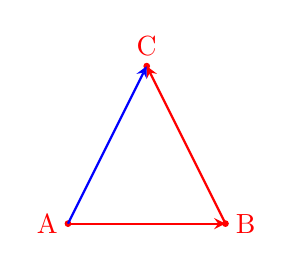
\begin{tikzpicture}[scale=1]
            \draw [red,thick,-stealth] (0,0) node[left] {A} -- (2,0) node [right] {B}; 
            \draw [fill, red] (0,0) circle (1 pt);
            \draw [fill, red] (2,0) circle (1 pt);
            \draw [fill, red] (1,2) circle (1 pt);
            \draw [red, thick, -stealth] (2,0) -- (1,2) node[above] {C};
            \onslide<2->{
                \draw [blue, thick, -stealth] (0,0) -- (1,2);
            }
        \end{tikzpicture}
    \end{center}

    \onslide<2-> {
        \begin{itemize}
            \item Para determinar o vetor \(\vec{x}=\vec{u}+\vec{v}+\vec{w}+\ldots\), tomam-se representantes consecutivos 
                (a origem de cada um coincidindo com a extremidade do anterior) e ''fecha-se o polígono''
            \item Se os representantes dos vetores a serem somados não forem consecutivos, basta encontrar 
                outros representantes
        \end{itemize}
    }
\end{frame}

\begin{frame}{Soma de vetores}

    Sejam \(\vec{u}\), \(\vec{v}\) e \(\vec{w}\) vetores quaisquer. Valem as propriedades básicas:

    \begin{itemize}
        \item \textbf{Propriedade associativa}:
            \((\vec{u}+\vec{v})+\vec{w}=\vec{u}+(\vec{v}+\vec{w})\)
        \item \textbf{Propriedade comutativa}: \(\vec{u}+\vec{v}=\vec{v}+\vec{u}\)
        \item \textbf{Elemento neutro}: \(\vec{u}+\vec{0}=\vec{u}\)
        \item \textbf{Elemento oposto}: \(\vec{u}+(-\vec{u})=\vec{0}\)
    \end{itemize}
    \pause
    A partir dessas propriedades básicas, podemos obter diversas propriedades derivadas, como por exemplo:
    \begin{itemize}
        \item \(\vec{x}+\vec{u}=\vec{y}+\vec{u} \textcolor{red}{\Rightarrow} \vec{x}=\vec{y}\)
        \item \(\vec{x}+\vec{u}=\vec{u} \textcolor{red}{\Rightarrow} \vec{x}=\vec{0}\)
        \item \(\vec{x}+\vec{u}=\vec{0} \textcolor{red}{\Rightarrow} \vec{x}=-\vec{u}\)
        \item \(\vec{x}+\vec{a}=\vec{b} \textcolor{red}{\Rightarrow} \vec{x}=\vec{b}-\vec{a}\)
        \item \(\vec{u}=\vec{v} \textcolor{red}{\Rightarrow} \vec{u}-\vec{v}=\vec{0}\)
    \end{itemize}
\end{frame}

\begin{frame}{Exemplo 1}
\begin{columns}

\begin{column}[t]{0.38\textwidth}

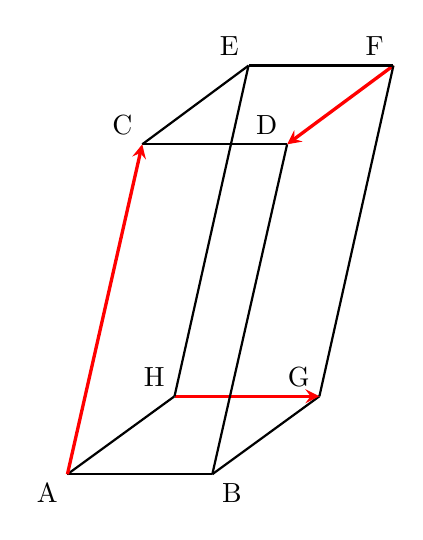
\begin{tikzpicture}[>=stealth]
    \coordinate (A) at (0.35,0.56);
    \coordinate (B) at (2.19,0.56);
    \coordinate (C) at (1.3,4.75);
    \coordinate (D) at (3.14,4.75);
    \coordinate (E) at (2.65,5.75);
    \coordinate (F) at (4.49,5.75);
    \coordinate (G) at (3.55,1.55);
    \coordinate (H) at (1.71,1.55);
    \draw [thick] (A) -- (B);
    \draw [thick] (B) -- (G);
    \draw [very thick, ->, red] (H) -- (G);
    \draw [thick] (H) -- (A);
    \draw [thick] (C) -- (D);
    \draw [very thick, ->, red] (F) -- (D);
    \draw [thick] (F) -- (E);
    \draw [thick] (E) -- (C);
    \draw [very thick,->, red] (A) -- (C);
    \draw [thick] (D) -- (B);
    \draw [thick] (H) -- (E);
    \draw [thick] (F) -- (G);
    \node [below left]  at (A) {A};
    \node [below right] at (B) {B};
    \node [above left]  at (C) {C};
    \node [above left]  at (D) {D};
    \node [above left]  at (E) {E};
    \node [above left]  at (F) {F};
    \node [above left]  at (G) {G};
    \node [above left]  at (H) {H};
\end{tikzpicture}
\end{column}

\begin{column}[t]{0.62\textwidth}
\begin{itemize}
    \item Sejam os vetores \(\vec{AC}\), \(\vec{HG}\) e \(\vec{FD}\)
    \item Vamos calcular \(\vec{AC}+\vec{HG}+\vec{FD}\)
    \item Temos que \(\vec{HG}=\vec{EF}\) (mesma direção, tamanho e sentido)
    \item Temos que \(\vec{AC}=\vec{HE}\) (mesma direção, tamanho e sentido)
\end{itemize}
\end{column}
\end{columns}

\end{frame}

\begin{frame}{Exemplo 1}
\begin{columns}

\begin{column}[t]{0.38\textwidth}

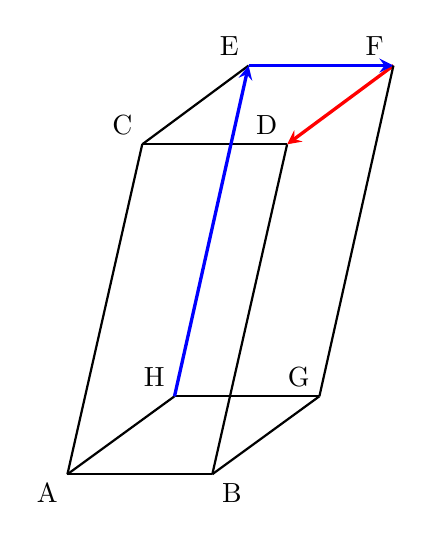
\begin{tikzpicture}[>=stealth]
    \coordinate (A) at (0.35,0.56);
    \coordinate (B) at (2.19,0.56);
    \coordinate (C) at (1.3,4.75);
    \coordinate (D) at (3.14,4.75);
    \coordinate (E) at (2.65,5.75);
    \coordinate (F) at (4.49,5.75);
    \coordinate (G) at (3.55,1.55);
    \coordinate (H) at (1.71,1.55);
    \draw [thick] (A) -- (B);
    \draw [thick] (B) -- (G);
    \draw [thick] (H) -- (G);
    \draw [thick] (H) -- (A);
    \draw [thick] (C) -- (D);
    \draw [very thick, ->, red] (F) -- (D);
    \draw [very thick, ->, blue] (E) -- (F);
    \draw [thick] (E) -- (C);
    \draw [thick] (A) -- (C);
    \draw [thick] (D) -- (B);
    \draw [very thick, ->, blue] (H) -- (E);
    \draw [thick] (F) -- (G);
    \node [below left]  at (A) {A};
    \node [below right] at (B) {B};
    \node [above left]  at (C) {C};
    \node [above left]  at (D) {D};
    \node [above left]  at (E) {E};
    \node [above left]  at (F) {F};
    \node [above left]  at (G) {G};
    \node [above left]  at (H) {H};
\end{tikzpicture}
\end{column}

\begin{column}[t]{0.62\textwidth}
\begin{itemize}
    \item Sejam os vetores \(\vec{AC}\), \(\vec{HG}\) e \(\vec{FD}\)
     \item Vamos calcular \(\vec{AC}+\vec{HG}+\vec{FD}\)
    \item Temos que \(\vec{HG}=\vec{EF}\) (mesma direção, tamanho e sentido)
    \item Temos que \(\vec{AC}=\vec{HE}\) (mesma direção, tamanho e sentido)
    \item Ou seja, podemos trocar \(\vec{AC}\) por \(\vec{HE}\) e \(\vec{HG}\) por \(\vec{EF}\)
    \item \textbf{Ou seja}:
    \[
    \vec{AC}+\vec{HG}+\vec{FD} = \vec{HE}+\vec{EF}+\vec{FD}
    \]
\end{itemize}
\end{column}
\end{columns}

\end{frame}

\begin{frame}{Exemplo 1}
\begin{columns}

\begin{column}[t]{0.38\textwidth}

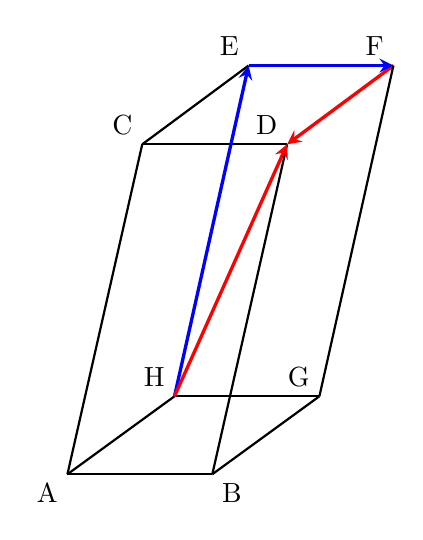
\begin{tikzpicture}[>=stealth]
    \coordinate (A) at (0.35,0.56);
    \coordinate (B) at (2.19,0.56);
    \coordinate (C) at (1.3,4.75);
    \coordinate (D) at (3.14,4.75);
    \coordinate (E) at (2.65,5.75);
    \coordinate (F) at (4.49,5.75);
    \coordinate (G) at (3.55,1.55);
    \coordinate (H) at (1.71,1.55);
    \draw [thick] (A) -- (B);
    \draw [thick] (B) -- (G);
    \draw [thick] (H) -- (G);
    \draw [thick] (H) -- (A);
    \draw [thick] (C) -- (D);
    \draw [very thick, ->, red] (F) -- (D);
    \draw [very thick, ->, blue] (E) -- (F);
    \draw [thick] (E) -- (C);
    \draw [thick] (A) -- (C);
    \draw [thick] (D) -- (B);
    \draw [very thick, ->, blue] (H) -- (E);
    \draw [thick] (F) -- (G);
    \node [below left]  at (A) {A};
    \node [below right] at (B) {B};
    \node [above left]  at (C) {C};
    \node [above left]  at (D) {D};
    \node [above left]  at (E) {E};
    \node [above left]  at (F) {F};
    \node [above left]  at (G) {G};
    \node [above left]  at (H) {H};

    \draw[very thick, ->, red] (H) -- (D);
\end{tikzpicture}
\end{column}

\begin{column}[t]{0.62\textwidth}
\begin{itemize}
    \item Sejam os vetores \(\vec{AC}\), \(\vec{HG}\) e \(\vec{FD}\)
    \item Vamos calcular \(\vec{AC}+\vec{HG}+\vec{FD}\)
    \item Temos que \(\vec{HG}=\vec{EF}\) (mesma direção, tamanho e sentido)
    \item Temos que \(\vec{AC}=\vec{HE}\) (mesma direção, tamanho e sentido)
    \item Ou seja, podemos trocar \(\vec{AC}\) por \(\vec{HE}\) e \(\vec{HG}\) por \(\vec{EF}\)
    \item \textbf{Ou seja}:
    \[
    \vec{AC}+\vec{HG}+\vec{FD} = \vec{HE}+\vec{EF}+\vec{FD}
    \]
    \item Finalmente, temos o vetor \(\vec{HD}\)...
\end{itemize}
\end{column}
\end{columns}

\end{frame}

\begin{frame}{Exemplo 2}
\begin{columns}

\begin{column}[t]{0.38\textwidth}

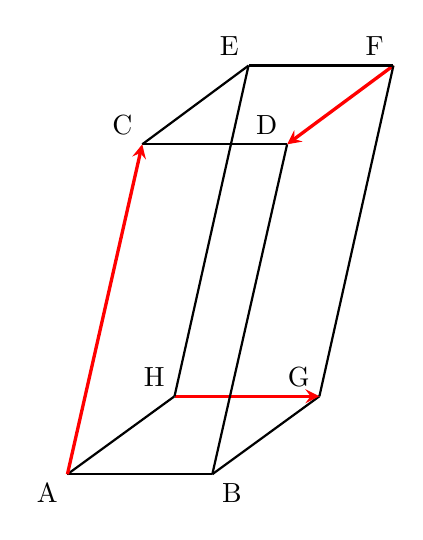
\begin{tikzpicture}[>=stealth]
    \coordinate (A) at (0.35,0.56);
    \coordinate (B) at (2.19,0.56);
    \coordinate (C) at (1.3,4.75);
    \coordinate (D) at (3.14,4.75);
    \coordinate (E) at (2.65,5.75);
    \coordinate (F) at (4.49,5.75);
    \coordinate (G) at (3.55,1.55);
    \coordinate (H) at (1.71,1.55);
    \draw [thick] (A) -- (B);
    \draw [thick] (B) -- (G);
    \draw [very thick, ->, red] (H) -- (G);
    \draw [thick] (H) -- (A);
    \draw [thick] (C) -- (D);
    \draw [very thick, ->, red] (F) -- (D);
    \draw [thick] (F) -- (E);
    \draw [thick] (E) -- (C);
    \draw [very thick,->, red] (A) -- (C);
    \draw [thick] (D) -- (B);
    \draw [thick] (H) -- (E);
    \draw [thick] (F) -- (G);
    \node [below left]  at (A) {A};
    \node [below right] at (B) {B};
    \node [above left]  at (C) {C};
    \node [above left]  at (D) {D};
    \node [above left]  at (E) {E};
    \node [above left]  at (F) {F};
    \node [above left]  at (G) {G};
    \node [above left]  at (H) {H};
\end{tikzpicture}
\end{column}

\begin{column}[t]{0.62\textwidth}
\begin{itemize}
    \item Sejam os vetores \(\vec{AC}\), \(\vec{HG}\) e \(\vec{FD}\)
    \item Vamos calcular \(\vec{AC}-\vec{HG}+\vec{FD}=\vec{AC}+(-\vec{HG})+\vec{FD}\)
    \item Temos que \(-\vec{HG}=\vec{BA}\) (mesma direção, tamanho e sentido oposto ao de \(\vec{HG}\))
    \item Temos que \(\vec{FD}=\vec{GB}\) (mesma direção, tamanho e sentido)
\end{itemize}
\end{column}
\end{columns}

\end{frame}

\begin{frame}{Exemplo 2}
\begin{columns}

\begin{column}[t]{0.38\textwidth}

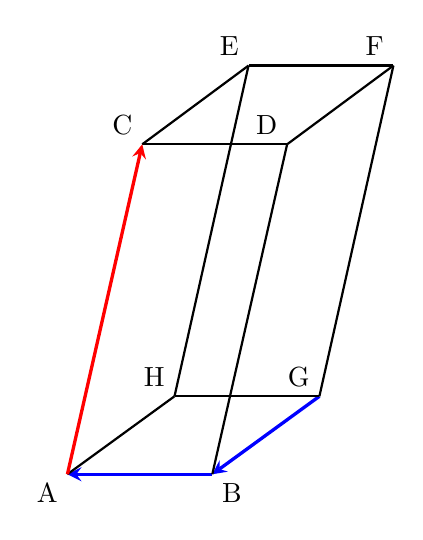
\begin{tikzpicture}[>=stealth]
    \coordinate (A) at (0.35,0.56);
    \coordinate (B) at (2.19,0.56);
    \coordinate (C) at (1.3,4.75);
    \coordinate (D) at (3.14,4.75);
    \coordinate (E) at (2.65,5.75);
    \coordinate (F) at (4.49,5.75);
    \coordinate (G) at (3.55,1.55);
    \coordinate (H) at (1.71,1.55);
    \draw [very thick, <-, blue] (A) -- (B);
    \draw [very thick, <-, blue] (B) -- (G);
    \draw [thick] (H) -- (G);
    \draw [thick] (H) -- (A);
    \draw [thick] (C) -- (D);
    \draw [thick] (F) -- (D);
    \draw [thick] (F) -- (E);
    \draw [thick] (E) -- (C);
    \draw [very thick,->, red] (A) -- (C);
    \draw [thick] (D) -- (B);
    \draw [thick] (H) -- (E);
    \draw [thick] (F) -- (G);
    \node [below left]  at (A) {A};
    \node [below right] at (B) {B};
    \node [above left]  at (C) {C};
    \node [above left]  at (D) {D};
    \node [above left]  at (E) {E};
    \node [above left]  at (F) {F};
    \node [above left]  at (G) {G};
    \node [above left]  at (H) {H};
\end{tikzpicture}
\end{column}

\begin{column}[t]{0.62\textwidth}
\begin{itemize}
    \item Sejam os vetores \(\vec{AC}\), \(\vec{HG}\) e \(\vec{FD}\)
    \item Vamos calcular \(\vec{AC}-\vec{HG}+\vec{FD}=\vec{AC}+(-\vec{HG})+\vec{FD}\)
    \item Temos que \(-\vec{HG}=\vec{BA}\) (mesma direção, tamanho e sentido oposto ao de \(\vec{HG}\))
    \item Temos que \(\vec{FD}=\vec{GB}\) (mesma direção, tamanho e sentido)
    \item Assim:
    \[
    \vec{AC}+(-\vec{HG})+\vec{FD} = \vec{AC}+\vec{BA}+\vec{GB}
    \]
\end{itemize}
\end{column}
\end{columns}

\end{frame}

\begin{frame}{Exemplo 2}
\begin{columns}

\begin{column}[t]{0.38\textwidth}

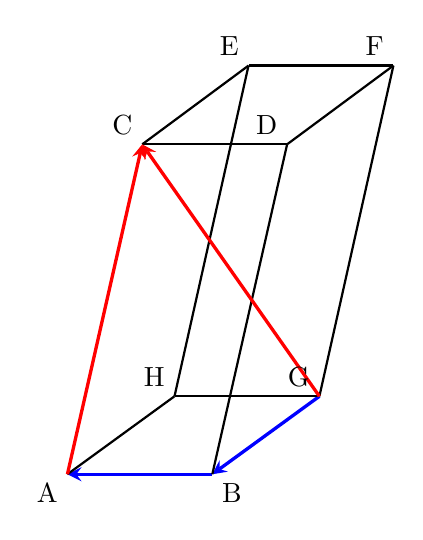
\begin{tikzpicture}[>=stealth]
    \coordinate (A) at (0.35,0.56);
    \coordinate (B) at (2.19,0.56);
    \coordinate (C) at (1.3,4.75);
    \coordinate (D) at (3.14,4.75);
    \coordinate (E) at (2.65,5.75);
    \coordinate (F) at (4.49,5.75);
    \coordinate (G) at (3.55,1.55);
    \coordinate (H) at (1.71,1.55);
    \draw [very thick, <-, blue] (A) -- (B);
    \draw [very thick, <-, blue] (B) -- (G);
    \draw [thick] (H) -- (G);
    \draw [thick] (H) -- (A);
    \draw [thick] (C) -- (D);
    \draw [thick] (F) -- (D);
    \draw [thick] (F) -- (E);
    \draw [thick] (E) -- (C);
    \draw [very thick,->, red] (A) -- (C);
    \draw [thick] (D) -- (B);
    \draw [thick] (H) -- (E);
    \draw [thick] (F) -- (G);
    \draw[very thick,->, red] (G) -- (C);
    \node [below left]  at (A) {A};
    \node [below right] at (B) {B};
    \node [above left]  at (C) {C};
    \node [above left]  at (D) {D};
    \node [above left]  at (E) {E};
    \node [above left]  at (F) {F};
    \node [above left]  at (G) {G};
    \node [above left]  at (H) {H};
\end{tikzpicture}
\end{column}

\begin{column}[t]{0.62\textwidth}
\begin{itemize}
    \item Sejam os vetores \(\vec{AC}\), \(\vec{HG}\) e \(\vec{FD}\)
    \item Vamos calcular \(\vec{AC}-\vec{HG}+\vec{FD}=\vec{AC}+(-\vec{HG})+\vec{FD}\)
    \item Temos que \(-\vec{HG}=\vec{BA}\) (mesma direção, tamanho e sentido oposto ao de \(\vec{HG}\))
    \item Temos que \(\vec{FD}=\vec{GB}\) (mesma direção, tamanho e sentido)
    \item Assim:
    \[
    \vec{AC}+(-\vec{HG})+\vec{FD} = \vec{AC}+\vec{BA}+\vec{GB}
    \]
    \item Finalmente, temos os vetor \(\vec{GC}\)
\end{itemize}
\end{column}

\end{columns}

\end{frame}


%\begin{frame}{Atividade para próxima aula}
%    Resolva o exercício 2-10 do livro texto (página 14), explicando os passos utilizados
%\end{frame}


